\section{Integrating scRNA-seq and CyTOF profiles}


We apply SCIM to integrate two sets of scRNA/CyTOF data,
one set corresponds to a melanoma tumor from the Tumor Profiler project \cite{irmisch2020}
and the other one to a human bone marrow sample from \citet{oetjen2018}.
The scRNA technology was chosen both times as the source technology, and the latent space is initialized by training a VAE.
SCIM is trained for 64 epochs to integrate the CyTOF technologies.
The discriminator is trained in both cases to classify the source technology.
We employed a semi-supervised strategy and use only 10\% of the cell-type labels to help orienting the latent space.
Bipartite matching is performed in both cases using $k=50$ and a null match penalty set to the $95^{th}$ percentile of edge costs.


\subsection{Integration of a melanoma sample}
A major motivation for this work is derived from the setting of the Tumor Profiler (TuPro) Consortium \cite{irmisch2020}.
This multi-center, multi-cancer study peforms a deep phenotyping of metastatic tumors from a real-life cohort, 
analyzing each sample with multiple technologies, including scRNA-sequencing \cite{tang2009} and Cytometry by Time Of Flight (CyTOF) \cite{bandura2009},
all of which are capable of dissecting the tumor microenvironment and providing single-cell level, complementary information about the sample of interest.
Although cell identity is lost throughout the experimental process, the cells profiled by both technologies stem from the same population
(i.e., were obtained from an aliquot of a common cell suspension), and can be thought of as being sampled from the same distribution of cells.

Here, we consider a melanoma sample from this study, and use SCIM to integrate CyTOF and scRNA-seq measurements to produce a more holistic cellular profile.

\subsubsection{Data Preparation}
\paragraph{CyTOF}
The patient's sample was profiled with CyTOF using a 41-markers panel designed for an in-depth characterization of the immune compartment of a sample.
Data preprocessing was performed following the workflow described in \cite{chevrier2017, chevrier2018}.
Cell-type assignment was performed using a Random Forest classifier trained on multiple manually gated samples.
To investigate the utility of SCIM, we considered a subset comprising B-cells and T-cells only, for a total of $n{=}135,334$ cells (Table \ref{tbl:tupro-dataset}).
This dataset is further referred to as \textit{target} dataset.

\paragraph{scRNA}
A second aliquot of the same patient sample was analyzed by droplet-based scRNA-sequencing using the 10x Genomics platform.
A detailed description of the data analysis workflow is beyond the scope of this work and will be published elsewhere.
In brief, standard QC-measures and preprocessing steps, such as removal of low quality cells, as well as filtering out mitochondrial, ribosomal and non-coding genes, were applied.
Expression data was library-size normalized and corrected for the cell-cycle effect.
Cell-type identification was performed using a set of cell-type-specific marker genes \cite{tirosh2016}.
Genes were then filtered to retain those that could code for proteins measured in CyTOF channels, the top 32 T-cell / B-cell marker genes, and the remaining most variable genes for a final set of 256.
The total number of B-cells and T-cells in this dataset amounts to $m{=}4,683$ (Table \ref{tbl:tupro-dataset}).
The scRNA dataset is used as \textit{source} dataset throughout the manuscript.

\begin{table}[ht]
    \centering
    \begin{tabular}{lrrrr}
    \toprule
    Dataset &  \# Markers &  \# Cells &  T Cells &  B Cells \\
    \midrule
    CyTOF &         41 &   135,334 &       70\% &       30\% \\
    scRNA &       256 &     4,683 &       73\% &       27\% \\
    \bottomrule
    \end{tabular}
    \caption{
        Characteristics of the preprocessed dataset derived from the melanoma sample.
    }
    \label{tbl:tupro-dataset}
\end{table}

\subsubsection{Model selection}
\paragraph{Autoencoders}
The training procedure for SCIM's autocoders is goverened by an adversarial loss function.
Model selection in this setting with real-world data is challenging since, as there is no metric that captures model performance, nor is there access to some ground truth data with which to evaluate.
To facilitate model selection, we employ a universal divergence estimator \cite{wang2009} to evaluate the quality of the integrated latent space (Supplmental Figure \ref{fig:tupro-train}).

This score measures how well two sets of points are mixed and it is computed pairwise between source and target technologies.
An optimization is defined as successful if the divergence and reconstruction errors are below the empirically set thresholds.
This allows the evaluation of many model settings at scale despite operating in the adversarial setting.
We find that performance depends on tuning $\beta$ and the learning rates for the discriminator and encoder/decoder networks, Supplementary Table \ref{tbl:ablation_menytek}.

%\begin{figure*}[htbp]
%    \centering
%    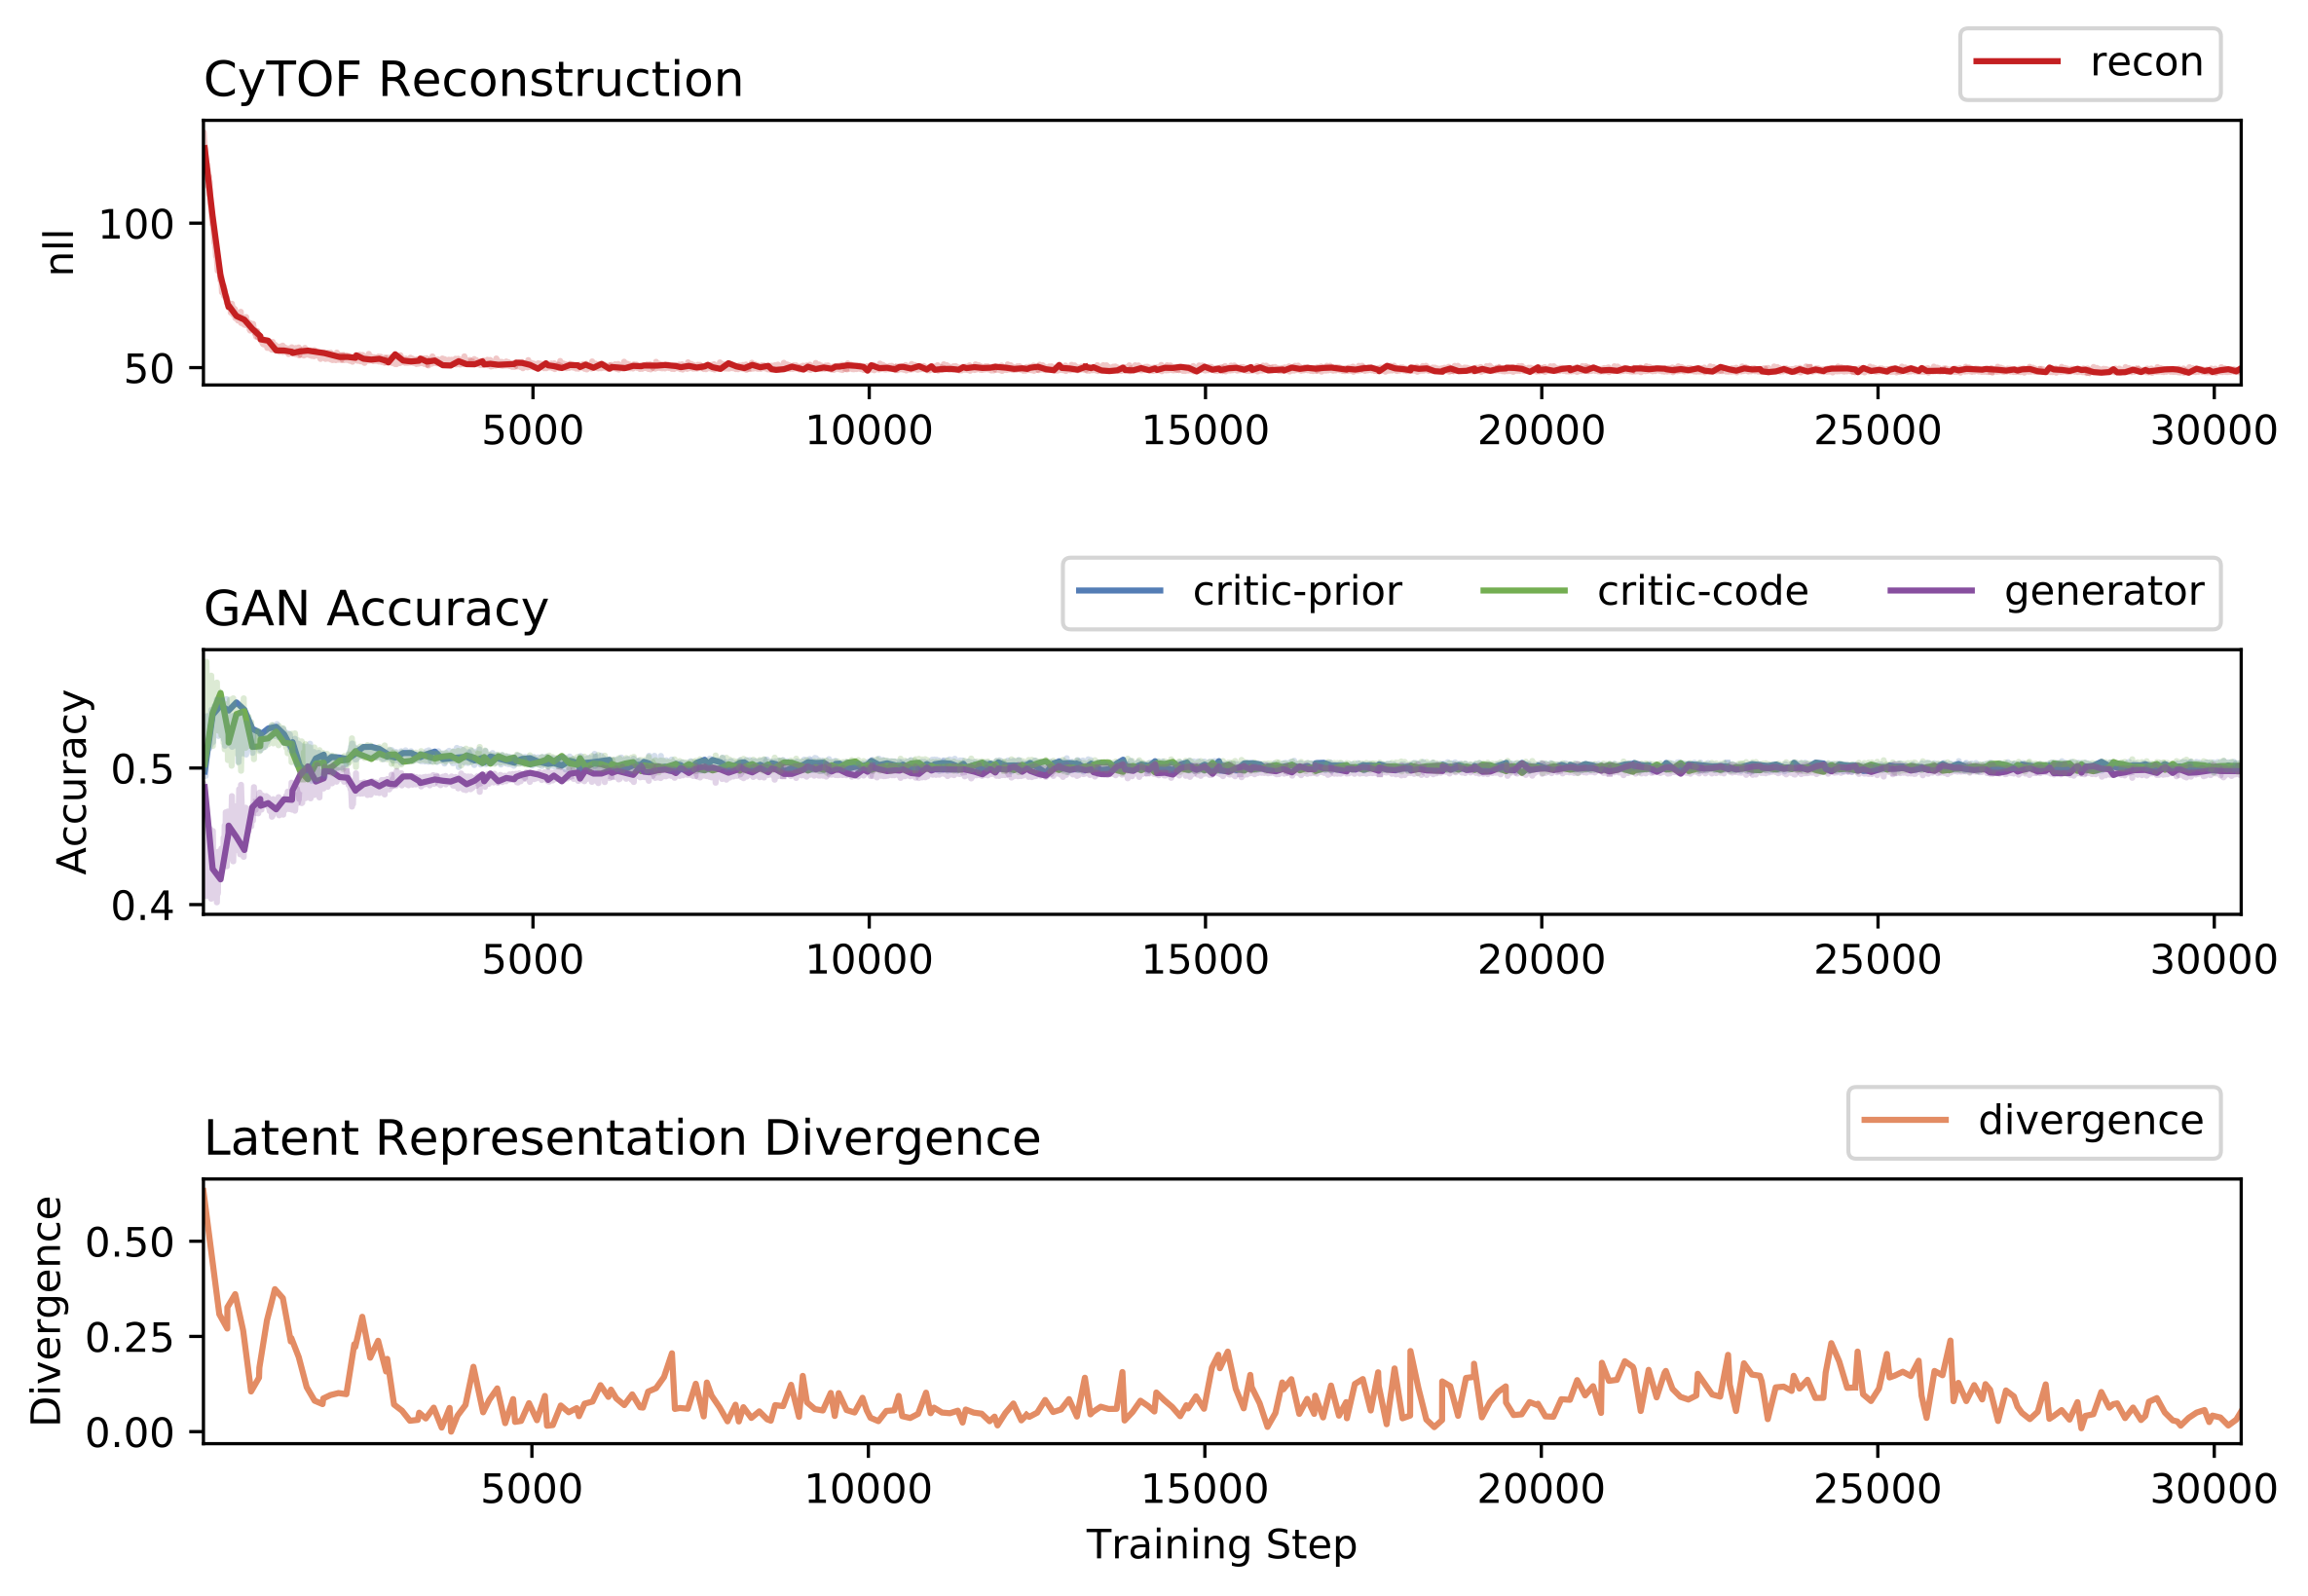
\includegraphics[width=0.95\textwidth]{figures/integration/menytek-train-scores}
%    \caption{
%        Training progress of SCIM on a melanoma sample.
%        The latent space is initialized by training a VAE on scRNA data.
%        SCIM integrates CyTOF representations into the latent space
%        defined by the scRNA codes.
%        The top panel shows the negative log-likelihood of the CyTOF reconstruction.
%        The middle panel shows the performance of the discriminator to correctly classify scRNA codes (critic-prior), CyTOF codes (critic-code), and the ability of the encoder to fool the discriminator, i.e., the misclassification accuracy (generator).
%        The bottom panel shows the divergence of the latent representations.
%        The model is able to converge quickly.
%However, the divergence score can fluctuate despite still fooling the discriminator.
%        Training took 2h 10min and had a peak memory consumption of 1068 MB.
%    }
%    \label{fig:tupro-train}
%\end{figure*}

%\begin{table}[h]
%\centering
%\begin{tabular}{rrrrrr}
%\toprule
%Censor & $\beta$ &  ${lr}_{\phi,\psi}$&  ${lr}_\gamma$ & Success &  \# runs \\
%\midrule
%0.00 &      16 &            0.0010 &  0.0010 &         14\% &           7 \\
%     &      16 &            0.0010 &  0.0005 &         14\% &           7 \\
%     &      16 &            0.0005 &  0.0005 &         10\% &          10 \\
%     &      16 &            0.0005 &  0.0010 &         10\% &          10 \\
%0.25 &      16 &            0.0010 &  0.0010 &         14\% &          14 \\
%     &      16 &            0.0005 &  0.0010 &         12\% &          17 \\
%     &      64 &            0.0001 &  0.0005 &          0\% &           7 \\
%     &      64 &            0.0001 &  0.0010 &          0\% &           7 \\
%0.75 &      16 &            0.0005 &  0.0010 &         17\% &           6 \\
%     &      32 &            0.0005 &  0.0005 &         12\% &           8 \\
%     &      16 &            0.0010 &  0.0005 &          8\% &          13 \\
%     &      64 &            0.0001 &  0.0005 &          0\% &           7 \\
%0.90 &      16 &            0.0005 &  0.0010 &         40\% &          10 \\
%     &      16 &            0.0010 &  0.0005 &         10\% &          10 \\
%     &      16 &            0.0005 &  0.0005 &          8\% &          12 \\
%     &      32 &            0.0010 &  0.0001 &          0\% &          10 \\
%0.95 &      32 &            0.0010 &  0.0001 &          0\% &           4 \\
%     &      64 &            0.0001 &  0.0005 &          0\% &           4 \\
%     &      64 &            0.0001 &  0.0010 &          0\% &           6 \\
%     &      32 &            0.0010 &  0.0010 &          0\% &           5 \\
%0.99 &      16 &            0.0005 &  0.0010 &         17\% &           6 \\
%     &      32 &            0.0010 &  0.0005 &          0\% &           6 \\
%     &      64 &            0.0001 &  0.0005 &          0\% &           4 \\
%     &      32 &            0.0010 &  0.0001 &          0\% &           6 \\
%\bottomrule
%\end{tabular}
%\caption{
%    Ablation study for training SCIM on the melanoma patient at several levels of semi-supervision.
%    Fraction censored is the fraction of labels removed during training.
%    The top 4 configurations for each level of semi-supervision is shown.
%    $\beta$ is the regularization strength of the adversarial loss.
%    Learning rates are the initial settings of the ADAM optimizer.
%    If the latent space divergence is below 0.3 and
%    the negative log-likelihood of the input under the reconstruction is below 47,
%    the training is determined to be a success. These values were chosen empirically.
%    We see that $\beta$ and optimizer learning rates were heavily influential on model success.
%}
%\label{tbl:ablation_menytek}
%\end{table}

\paragraph{Bi-partite matching is scalable}
Due to the large number of cells profiled with each individual technology per sample, we precede our bipartite matching with a kNN search.
This reduces the problem complexity by \textit{a priori} discarding redundant edges in the graph.
Experiments on the real-world melanoma sample investigating the level of sparsity, governed by a hyperparameter \textit{k}, show that using even a small number of neighbors provides good matching accuracy and performance saturates past $k>100$ (see Supplemental Figure~\ref{fig:matching_accuracy_log10_uni}, Supplemental Table~\ref{tbl:menytek_tune_k_uni}).
This is in line with our expectations since a match to an extremely distant neighbor is hard to justify.
In order to maintain a high degree of sparsity, without sacrificing matching accuracy, we use $k=50$ in all further experiments.

%\begin{figure*}[h]
%    \centering
%    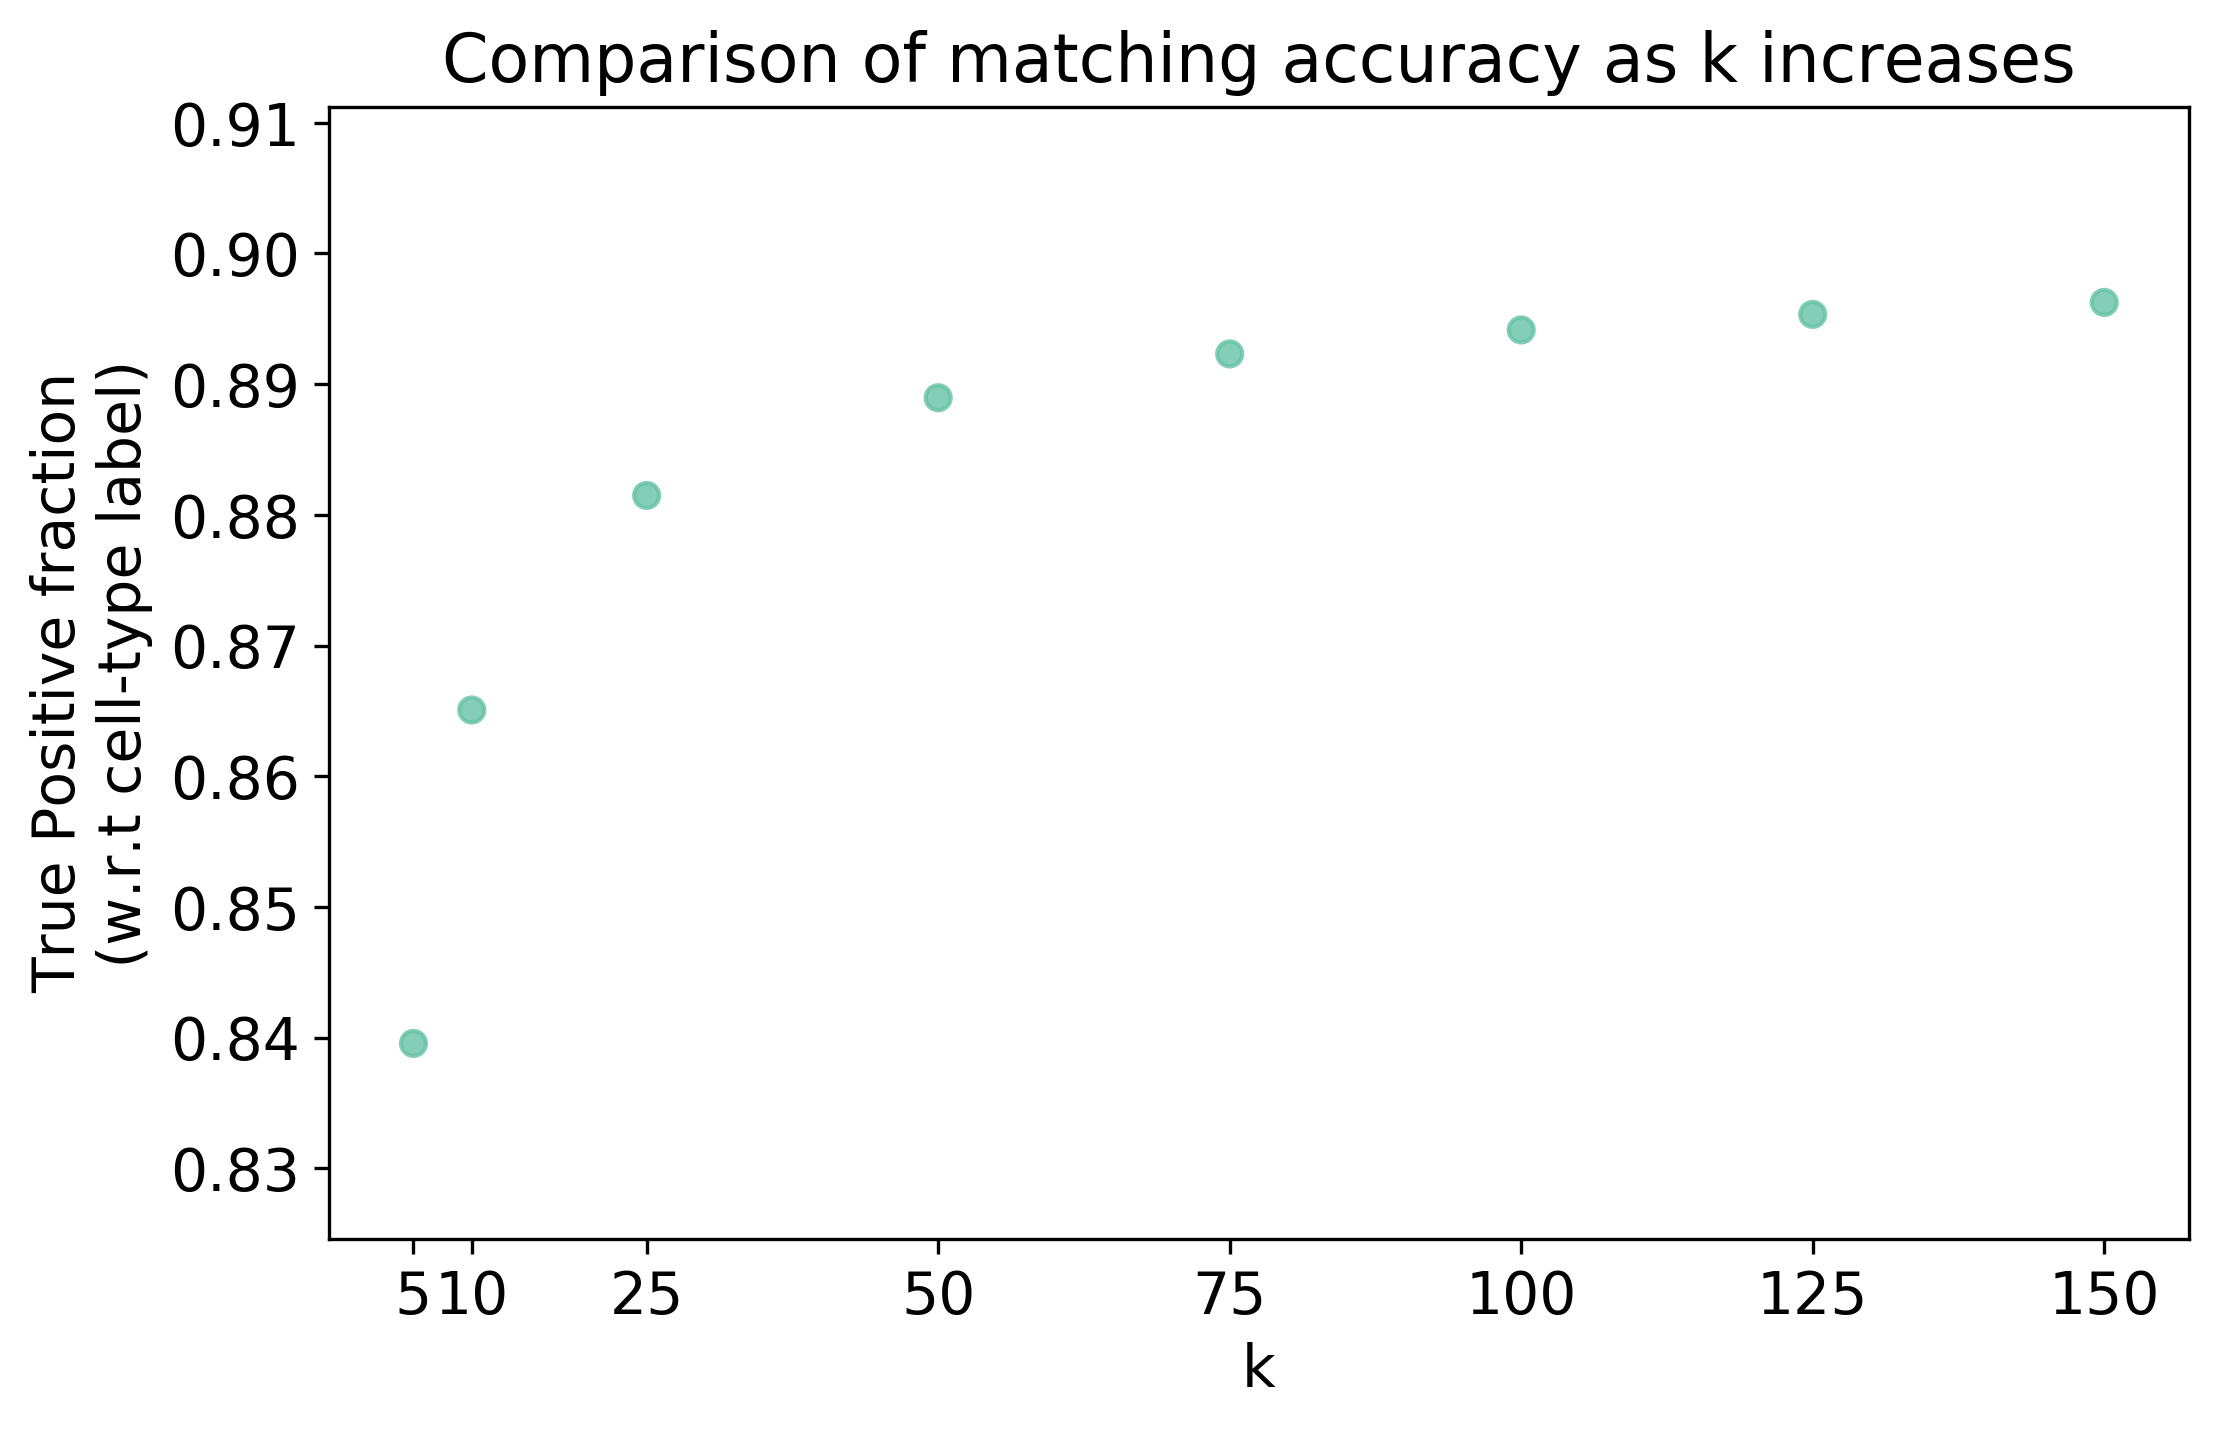
\includegraphics[width=0.85\textwidth]{figures/integration/matching-tune-k-unicapacity.png}
%    \caption{Comparison of matching accuracy, with respect to cell-type label as less sparsity of connections, is imposed on the Tumor Profiler data.
%The number of considered Nearest Neighbors \textit{k} is indicated on the x-axis, and the fraction of true positive matches, with respect to cell-type label, is depicted on the y-axis.
% The accuracy level saturates with $k=100$.}
%    \label{fig:matching_accuracy_log10_uni}
%\end{figure*}
%
%\begin{table*}[h]
%\centering
%\begin{tabular}{lrr}
%\toprule
%{} &  CPU time [s] &  Max Memory [Mb] \\
%k   &               &                  \\
%\midrule
%5   &       1,492.67 &          1,674.94 \\
%10  &       2,803.33 &          2,456.27 \\
%25  &       7,723.67 &          4,690.05 \\
%50  &       7,441.33 &          8,740.34 \\
%75  &      12,656.00 &         12,344.52 \\
%100 &      17,331.00 &         17,002.75 \\
%125 &      26,047.00 &         20,612.78 \\
%150 &      33,718.00 &         24,222.75 \\
%\bottomrule
%\end{tabular}

%\caption{Memory usage and computation time of the bipartite matching as \textit{k} hyperparameter in kNN search increases.
%The values were obtained on the whole TuPro dataset using the MCMF algorithm on an extended graph. %, as described in section \ref{graph_extensions}.
%The cost of matching to the null node was set to 95th percentile, and a union of connections obtained from kNN graphs with \textit{k} indicated in the first column was used for matching.
%The memory and time reports were averaged across three independent runs.}
%\label{tbl:menytek_tune_k_uni}
%\end{table*}

\subsection{SCIM Pairs Cells Across scRNA and CyTOF in a Melanoma Sample}
The bipartite matching on the latent codes has a 90\% accuracy in recovering the cell-type label, calculated as the fraction of true positives over all matches.
A more fine-grained visual evaluation is performed by inspecting the matches on a tSNE embedding of the integrated latent space marked by grey lines, Figure \ref{fig:tupro-tsne-uni}.
Given different cell-type proportions in the data, a certain number of mismatches is expected, which corresponds to the lines joining points across the two cell types.
The latent representation is explored thoroughly as 98\%, and 99.9\% of cells are matched to their analogs, from CyTOF and scRNA datasets, respectively.
To evaluate the latent space matching further, we used a more fine-grained information of marker expression correlation, to quantitatively assess the latent-space matching quality.
We used the correlation coefficients between the expression of immunomarkers \textsc{CD20} and \textsc{CD3}.
Both markers are characteristic for a subset of our data, as they are used to differentiate B-cells and T-cells, respectively.
We found that matching using shared latent representations provides relatively high correlation coefficients
(Pearson: 0.63 \textsc{CD20} and 0.51 for \textsc{CD3} marker, see Supplemental Figure~\ref{fig:tupro-marker-correlation-uni}),
given the expected low correlation between RNA expression and protein abundance.

\begin{figure*}[htbp]
    \centering
    \includegraphics[width=0.95\textwidth]{figures/integration/tsne-matched-unicapacity.png}
    \caption{
    Integrated latent space and matches of scRNA and CyTOF cells from a melanoma sample from the Tumor Profiler Consortium.
    Discriminators are semi-supervised using 10\% of the cell-type labels.
    Cells are colored by their cell-type label and shaded by their technology (dark shades: CyTOF, light shades: scRNA).
    Matches produced by SCIM are represented by grey lines connecting cells.
    tSNE embeddings \cite{maaten2008} are computed on the whole dataset and then 10,000 matched pairs are sampled at random for visualization.}
    \label{fig:tupro-tsne-uni}
\end{figure*}


%\begin{figure*}[htbp]
%    \centering
%    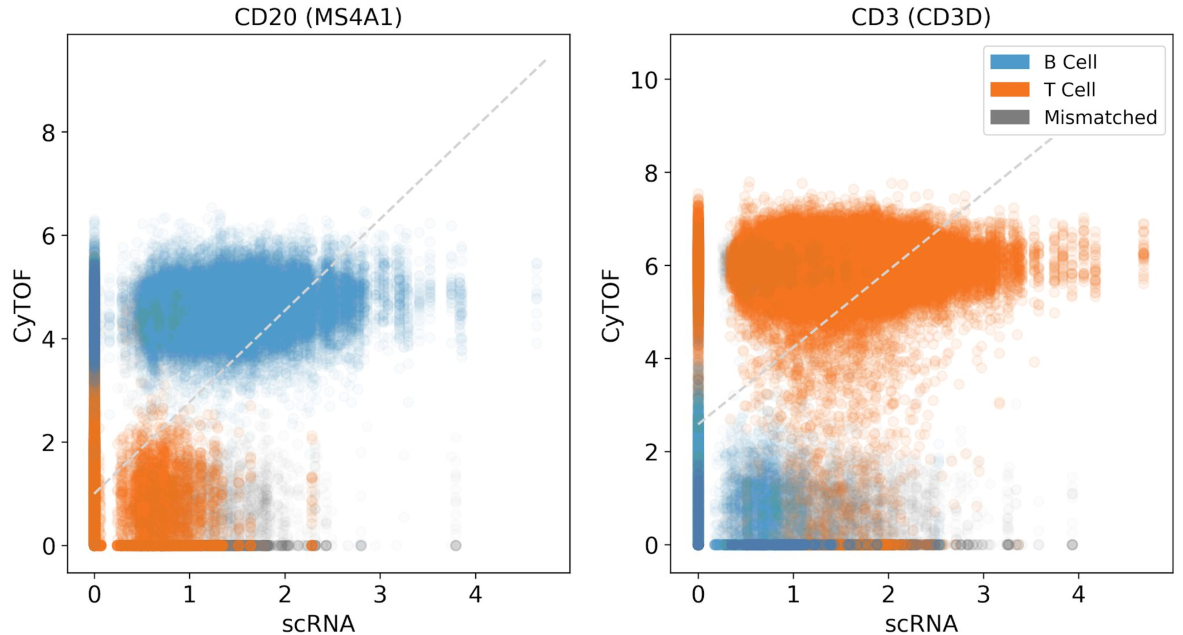
\includegraphics[width=0.65\textwidth]{figures/integration/gene_protein_correlation_unicapacity}
%    \caption{
%      \textit{CD20} and \textit{CD3} marker abundances measured with scRNA (gene, x-axis) and CyTOF (protein, y-axis) in a melanoma sample from the Tumor Profiler Consortium.
%      The values on the axes represent normalized expression.
%      Colors (blue, orange) represent cell types (B-cell, T-cell) while grey marks mismatches with respect to the cell-type label.
%      The linear regression line is depicted by a dashed light grey line.
%      Pearson's correlation coefficient equals 0.63 and 0.51 for CD20 and CD3, respectively.
%      Spearman's correlation coefficient amounts to 0.55 and 0.42, for CD20 and CD3, respectively.
%    }
%    \label{fig:tupro-marker-correlation-uni}
%\end{figure*}


\subsection{Integration of a human bone marrow sample}
\citet{oetjen2018} used several bulk and single-cell technologies to comprehensively characterize human bone marrow.
The data was obtained from 20 healthy donors, whereas all data modalities were acquired for 8 samples.
For our application we consider the single-cell transcriptome profile as well as CyTOF measurements of sample \textit{O} from this dataset, that were carried out with the objective of describing in detail a T-cell~population.
The data was preprocessed as described by \citet{oetjen2018}.
A subpopulation of CD8 naive T-cells was filtered out due to a very small number of cells.
The preprocessed data of the analyzed sample included several T-cell~subtypes, Table \ref{tbl:oetjen-dataset}.

\begin{table}[h]
    \centering
    \begin{tabular}{lrrrrr}
    \toprule
    Dataset &  \# Markers &  \# Cells &  CD8 effector &  CD4 naive & CD4 memory  \\
    \midrule
    CyTOF &         34 &   98,799 &       57\% &       26\% & 17\% \\
    scRNA &       256 &     2,388 &       46\% &       31\% & 23\% \\
    \bottomrule
    \end{tabular}
    \caption{
        Characteristics of the preprocessed dataset derived from the human bone marrow sample. 
    }
    \label{tbl:oetjen-dataset}   
\end{table}

We use SCIM to integrate T-cells~derived from one sample in the Human Bone Marrow study, profiled with scRNA and CyTOF technologies.
The tSNE embedding based on the latent space codes implies good integration across technologies while preserving the cell-subtype structure Supplemental Figure~\ref{fig:oetjen_tsne_uni}.
We evaluate the quality of matches using fine-grained labels indicating one of the T-cell subtypes identified in gating: CD8 effector, CD4 naive, CD4 memory.
In a fully supervised approach, using the labels to orient the latent space, we achieve an accuracy of $83\%$ with  less than $8\%$ of matches directed to the null node.
Nevertheless, when utilizing only $10\%$ of the labels in the semi-supervised approach, we note only a slight drop in performance, obtaining $78\%$ correct matches with less than $8\%$ of cells directed to the null node.
Evaluating on higher-level labels of CD8 vs.
CD4 T-cells~improves the accuracy to $91\%$ and $86\%$ for the fully supervised and semi-supervised approach, respectively.
As expected, distinguishing cellular subtypes (e.g., CD4 naive versus CD4 memory) is more challenging due to high similarity between the cell populations, but overall SCIM is capable of accurately recovering even such subtle differences between cell types and states.

%\begin{figure*}[htb]
%    \centering
%    \includegraphics[width=0.85\textwidth]{figures/integration/oetjen-tsne-matched-unicapacity.png}
%    \caption{
%    A tSNE embedding (perplexity=30) of the integrated latent space with cell matches indicated by the grey lines.
%    The shared representation was obtained in a semi-supervised fashion, utilizing 10\% of the cell-type labels to orient the latent space. 10,000 matched pairs were sampled at random for the plot.
%    Colors (blue, green, orange) represent T-cell subtypes (CD8 effector, CD4 naive, CD4 memory), and color shades correspond to the profiling technology (light: scRNA, dark: CyTOF).}
%    \label{fig:oetjen_tsne_uni}
%\end{figure*}
